\documentclass[12pt,a4paper,openany]{report}
\usepackage[a4paper,margin=1in]{geometry}
\usepackage[T1]{fontenc}
\usepackage[utf8]{inputenc}
\usepackage{mathptmx}
\usepackage{setspace}
\usepackage{graphicx}
\usepackage{float}
\usepackage{booktabs}
\usepackage{array}
\usepackage{tabularx}
\usepackage{longtable}
\usepackage{xcolor}
\usepackage{hyperref}
\usepackage{caption}
\usepackage{tikz}
\usetikzlibrary{arrows.meta,positioning,shapes.geometric}
\usepackage{listings}
\usepackage{fancyhdr}
\usepackage{titlesec}
\usepackage{enumitem}
\usepackage{url}
\usepackage{placeins}

\hypersetup{colorlinks=true, linkcolor=black, urlcolor=blue, citecolor=black}
\onehalfspacing
\raggedbottom
\setlength{\parindent}{0pt}
\setlength{\parskip}{6pt}
\renewcommand{\arraystretch}{1.15}
\captionsetup{font=bf, labelfont=bf}
\urlstyle{same}

\definecolor{codegray}{RGB}{246,248,250}
\definecolor{codeborder}{RGB}{210,215,220}
\lstdefinestyle{reportcode}{
  backgroundcolor=\color{codegray},
  basicstyle=\ttfamily\small,
  breaklines=true,
  frame=single,
  framerule=0.4pt,
  rulecolor=\color{codeborder},
  columns=fullflexible,
  keepspaces=true,
  showstringspaces=false,
  tabsize=2
}
\lstset{style=reportcode}

\pagestyle{fancy}
\fancyhf{}
\fancyhead[L]{23AIML049}
\fancyhead[R]{Agentic Requirement Analyzer -- Internship Report}
\fancyfoot[L]{CSPIT, CHARUSAT}
\fancyfoot[C]{\thepage}
\fancyfoot[R]{Department of AIML}
\renewcommand{\headrulewidth}{0.4pt}
\renewcommand{\footrulewidth}{0.4pt}
\setlength{\headheight}{15pt}

\titleformat{\chapter}[display]
  {\normalfont\bfseries\centering\Large}
  {CHAPTER \thechapter}
  {0.5em}
  {\Large}
\titlespacing*{\chapter}{0pt}{-5pt}{14pt}
\titleformat{\section}{\normalfont\bfseries\large}{\thesection}{1em}{}
\titleformat{\subsection}{\normalfont\bfseries}{\thesubsection}{1em}{}

\newcommand{\reporttitle}{AGENTIC REQUIREMENT ANALYZER}
\newcommand{\subtitle}{Autonomous Multi-Agent AI System for Software Requirement Analysis and User Story Generation}
\newcommand{\student}{HARI PATEL}
\newcommand{\rollno}{23AIML049}
\newcommand{\internalguide}{Prof. Hardik Jaiswal}
\newcommand{\externalguide}{Mr. Pallav Mamtora}
\newcommand{\externaltitle}{CEO}
\newcommand{\company}{Techmicra IT Solutions}
\newcommand{\hod}{Dr. Nirav Bhatt}


\begin{document}
\pagestyle{fancy}
\setcounter{page}{4}

% ===== original PDF page 13 (report page 4) =====
\setcounter{chapter}{2}\setcounter{section}{1}\setcounter{table}{1}
\section{Non-Functional Requirements}
\begin{table}[H]
\centering
\caption{Non-Functional Requirements of the System}
\label{tab:nonfunctional}
\begin{tabularx}{\textwidth}{|>{\raggedright\arraybackslash}p{3.6cm}|X|}
\hline
\textbf{Quality Attribute} & \textbf{Implementation Direction} \\
\hline
Reliability & Every agent degrades gracefully -- a failed LLM call or malformed JSON response falls back to an empty result and is logged, instead of crashing the pipeline. \\
\hline
Modularity & Each agent is a self-contained function with its own prompt, taking and returning a shared pipeline state, so agents can be built, tested and debugged independently. \\
\hline
Explainability & LangGraph's explicit state-machine model was chosen over a more autonomous framework (e.g. CrewAI) so that each agent hand-off is deterministic and traceable. \\
\hline
Usability & A React frontend shows pipeline progress and renders the final report in a readable, sectioned layout rather than raw JSON. \\
\hline
Persistence & Past analysis runs are stored in SQLite so a report is not lost after the browser session ends. \\
\hline
\end{tabularx}
\end{table}

\section{Technology Stack}
\begin{table}[H]
\centering
\caption{Technology Stack Summary}
\label{tab:techstack}
\begin{tabularx}{\textwidth}{|p{3.2cm}|X|}
\hline
\textbf{Area} & \textbf{Technologies} \\
\hline
Orchestration & LangGraph \texttt{StateGraph} (six nodes, linear edges) \\
\hline
Language Model & Groq API (llama-3.3-70b-versatile; openai/gpt-oss-120b for the final test runs) \\
\hline
Backend & Python 3.11, FastAPI \\
\hline
Frontend & React 18, Tailwind CSS \\
\hline
Document Parsing & pypdf (PDF), python-docx (DOCX) \\
\hline
Ambiguity Detection & Sentence-Transformers embeddings, FAISS similarity search \\
\hline
Persistence & SQLite \\
\hline
Version Control & Git and GitHub \\
\hline
\end{tabularx}
\end{table}

% ===== original PDF page 14 (report page 5) =====
\clearpage
\setcounter{chapter}{2}\setcounter{table}{0}\setcounter{figure}{0}
\chapter{SYSTEM ARCHITECTURE}

\section{Pipeline Overview}
\vspace{0.25cm}
The system is built around a shared pipeline state that passes through six
agents in a fixed sequence. The pipeline is implemented as a compiled
LangGraph \texttt{StateGraph}~[2] in \texttt{backend/graph.py}: each agent is a node,
the nodes are joined by linear edges from \texttt{START} to \texttt{END}, and the
\texttt{errors} field uses an additive reducer so that warnings from every
agent are retained. Each agent reads the fields it needs and returns only
the fields it owns, which keeps intermediate output traceable.
Figure~\ref{fig:architecture} shows the complete pipeline.

\begin{figure}[H]
\centering
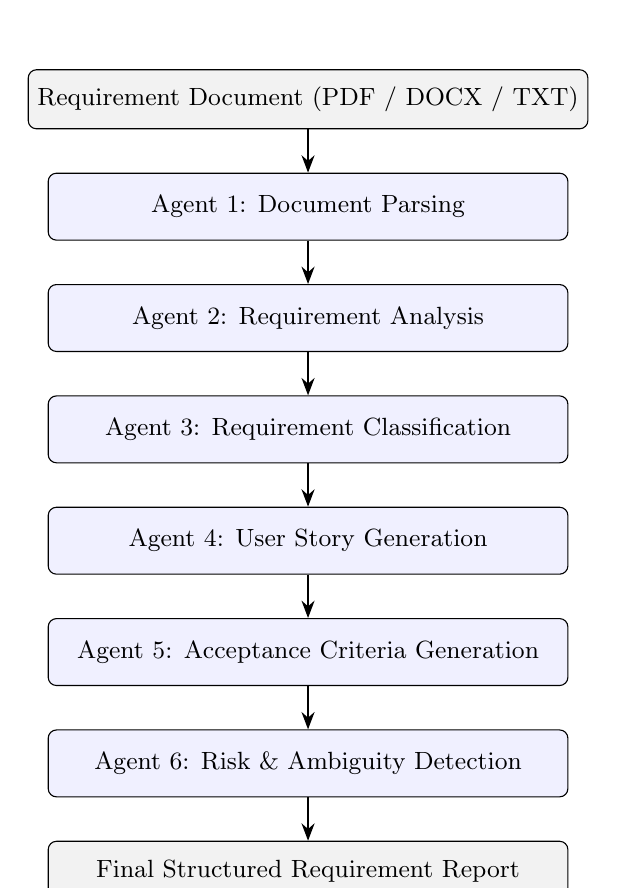
\begin{tikzpicture}[
  node distance=0.55cm and 0.9cm,
  every node/.style={font=\small},
  box/.style={draw, rounded corners=3pt, fill=blue!6, minimum width=6.6cm, minimum height=0.85cm, align=center},
  io/.style={draw, rounded corners=3pt, fill=gray!10, minimum width=6.6cm, minimum height=0.75cm, align=center},
  arr/.style={-{Stealth[length=2.2mm]}, thick}
]
\node[io] (doc) {Requirement Document (PDF / DOCX / TXT)};
\node[box, below=of doc] (a1) {Agent 1: Document Parsing};
\node[box, below=of a1] (a2) {Agent 2: Requirement Analysis};
\node[box, below=of a2] (a3) {Agent 3: Requirement Classification};
\node[box, below=of a3] (a4) {Agent 4: User Story Generation};
\node[box, below=of a4] (a5) {Agent 5: Acceptance Criteria Generation};
\node[box, below=of a5] (a6) {Agent 6: Risk \& Ambiguity Detection};
\node[io, below=of a6] (report) {Final Structured Requirement Report};
\draw[arr] (doc) -- (a1);
\draw[arr] (a1) -- (a2);
\draw[arr] (a2) -- (a3);
\draw[arr] (a3) -- (a4);
\draw[arr] (a4) -- (a5);
\draw[arr] (a5) -- (a6);
\draw[arr] (a6) -- (report);
\end{tikzpicture}
\caption{LangGraph pipeline architecture of the Agentic Requirement Analyzer.}
\label{fig:architecture}
\end{figure}

% ===== original PDF page 15 (report page 6) =====
\clearpage
\setcounter{page}{6}\setcounter{section}{1}
\section{Shared Pipeline State}
Every agent communicates through a single \texttt{PipelineState}
structure rather than passing ad-hoc arguments between functions. This
was one of the first design decisions made in the project, since it keeps
every agent independently testable.

\begin{lstlisting}
class PipelineState(TypedDict):
    raw_text: str
    filename: str
    actors: list[str]
    features: list[str]
    constraints: list[str]
    functional_requirements: list[str]
    non_functional_requirements: list[str]
    user_stories: list[dict]          # {feature, story, priority}
    acceptance_criteria: list[dict]   # {story_ref, given, when, then}
    risks: list[dict]                 # {requirement, reason, suggestion}
    ambiguities: list[dict]           # {requirement, reason, suggestion}
    errors: list[str]
\end{lstlisting}

\section{Agent Responsibilities}
\begin{longtable}{|p{3.3cm}|p{9.8cm}|}
\caption{Agent Responsibilities in the Pipeline}\\
\hline
\textbf{Agent} & \textbf{Responsibility} \\
\hline
Document Parsing & Detects the uploaded file type and extracts clean text, joining broken lines and stripping whitespace left over from PDF extraction. \\
\hline
Requirement Analysis and Classification & Reads the parsed text to identify actors, system features, and constraints, then classifies them into functional and non-functional requirements. \\
\hline
User Story Generation & Converts each functional requirement into an Agile user story with a priority level. \\
\hline
Acceptance Criteria Generation & Produces Given/When/Then acceptance criteria for every generated user story. \\
\hline
Risk \& Ambiguity Detection & Embeds each requirement, compares it against a seed corpus of known-vague phrases using FAISS, and asks the LLM to confirm the issue and suggest a concrete fix. \\
\hline
\end{longtable}
\end{document}
